\section{Existing work}

As I am now three years into my PhD, my research builds on significant prior work. First and foremost, my CORGIS project has already been used in several introductory programming experiences, and seen publication at multiple venues, including two very successful workshops.
My primary research project for the first two years of my dissertation led to CORGIS: Collections of Real-time, Giant, Interesting, Situated Datasets.
This project's goal is to make simplistic data sources available to learners early in their programming experience, so that they can explore Big Data Science contexts.

\subsection{Technical Infrastructure}

\begin{wrapfigure}{R}{0.5\textwidth}
    \begin{center}
			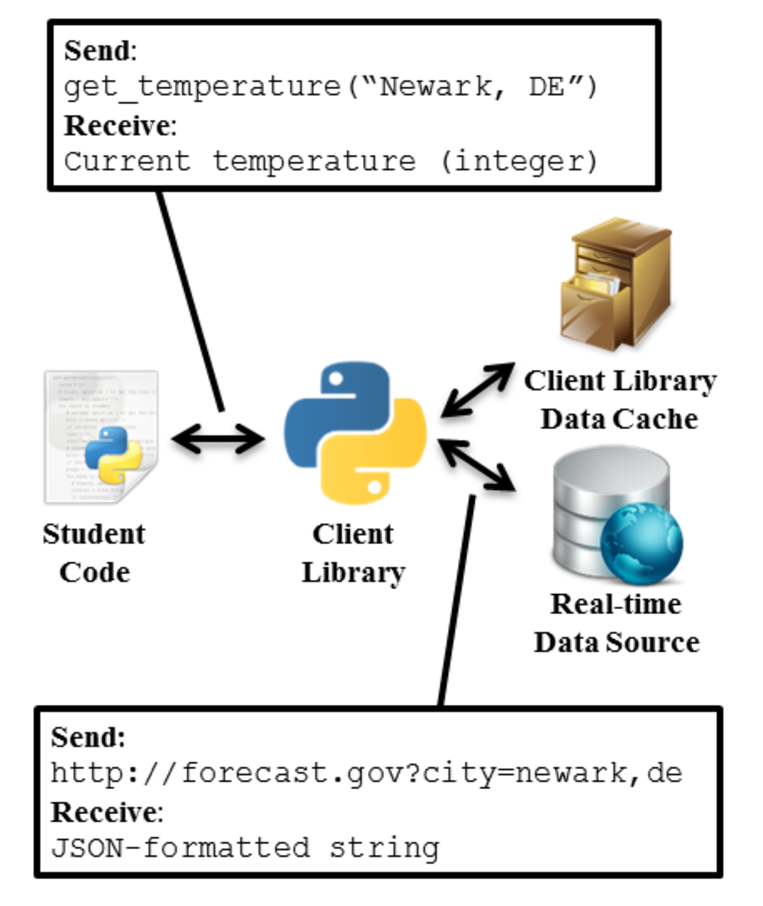
\psfig{file=images/rtw-client-library.eps, width=\linewidth}
			%\includegraphics[width=0.48\textwidth]{"images/rtw-client-library"}
    \end{center}
    \vspace{-\bigskipamount}
    \caption{RealTimeWeb Client Library Architecture}
    \label{fig-cla}
\end{wrapfigure}

The foundation of this proposal rests on prior work developing the RealTimeWeb project, a software architecture framework that provides introductory programming students with an easy way to access and manipulate distributed real-time data\cite{bart-transforming}.
Real-time data is a specific branch of Big Data -- specifically, high velocity data.

As our focus shifts from real-time data to datasets in general, we have renamed our overarching project from RealTimeWeb to CORGIS. Our work is now available at \url{http://think.cs.vt.edu/corgis/}. As a successor to the RealTimeWeb project, CORGIS retains all the previously developed libraries for accessing high velocity data; however, it also contains our new libraries for working with high volume data.
These libraries are paired with potential assignments and helpful documentation for deployment.
Long term, we intend to gather and disseminate data on the success of these libraries, with the hopes to establish a community of developers and educators that create new resources.
For clarity's sake, we use the name RealTimeWeb to refer to the architecture we have developed to rapidly connect to high velocity data streams.

At the heart of our project are carefully engineered, open-source client libraries through which students can access the data provided by real-time web services.
We provide client libraries for a number of data sources, such as business reviews from Yelp, weather forecasts from the National Weather Service, and social content from link-sharing site Reddit.com.
Each of these client libraries is in turn available for three common beginner languages: Java, Python, and Racket. 
These libraries do more than just streamline the process of accessing distributed data, however; each library is built with a persistence layer that enables the library to work without an internet connection.
Not only does this ensure that students without a solid internet connection can maintain productivity, it also simplifies developing unit tests. 
In fact, this technical scaffolding for the students circumvents most of the difficulties of distributed computing, including HTTP access, data validation, and result parsing.
Figure \ref{fig-cla} demonstrates the architecture used in our libraries.

The persistence layer is implemented using a caching mechanism, but not a traditional one.
In a conventional caching system, the result of every call made to the external service is memoized using a key-value store, often with a timestamp in order to expire out-of-date data.
In our caching system, an instructor preloads the cache with a sequence of data values for each expected call to the external service.
Although this limits the number of possible calls to the external service, it improves the consistency of the experience.
Instructors can specify policies for how the system returns data -- if the cache runs out, it could restart with the initial result, a developer-specified ``empty'' result, or repeatedly return the final result.
For example, consider the United States Geological Services' Earthquake data stream, which exposes a function to retrieve a list of earthquakes around the world for a given time period (e.g., past hour, past day, past week, etc.). 
The instructor could provide a cache to simulate a period of high seismic activity, returning a large number of earthquakes every time the function is called.
If the user exhausts the data in the cache, it might be programmed to return an empty list, signaling no further activity.

Our High Volume libraries often work by providing sampled versions of the data internally, so that students can work with faster, representative subsets.
Then, when they are ready for full deployment, they can switch to a ``full production'' mode -- trading speed for quality. 
Most of the work in developing these libraries is organizing the sampled data to load into memory and get processed as quickly and naturally as possible.

An alternative scheme for distributed High Volume libraries uses a more traditional caching strategy -- assuming that the data source is largely static, requests are cached locally.
This caching is typically done using a simple key-value store on the local filesystem.
Limits can be set on the size or lifespan of the data in the cache, allowing the system to update itself according to the velocity of the external data service.
Using open-source REST API generating tools such as Eve~\cite{Eve}, existing high volume datasets can be quickly transformed into distributed datasets, alleviating the issues of data storage and transmission.

\subsection{Semi-Automatic Library Generation}

Our client libraries are easily available through a curated, online gallery; each library is designed to be quickly adapted to instructors' specific academic desires. 
This gallery also provides a tool for rapidly prototyping new libraries based on our framework.
As an open-source project, we encourage collaborators to explore and extend the tools that we have created.

The process of connecting to online data sources is fairly uniform: performing an HTTP request to a URL returns formatted data (typically JSON or XML). 
This information must then be parsed into native data structures, and then filtered and transformed into an appropriate domain object using the language's proper construct (e.g., structs for Racket, classes for Java).
We've established a JSON-based client library specification file format that can be compiled to appropriate source code in each of the three target languages using the modern templating language Jinja2. 
This compiler can be easily extended to new languages by providing a template.
This specification format has two major components: the functions, which connect to the relevant URL endpoints, and the domain objects, that are generated from a successful HTTP request. 
This open-source tool has been used to successfully and rapidly develop a number of the existing client libraries.

\subsection{Contextualizing with CORGIS}

\begin{figure}
		\begin{center}
				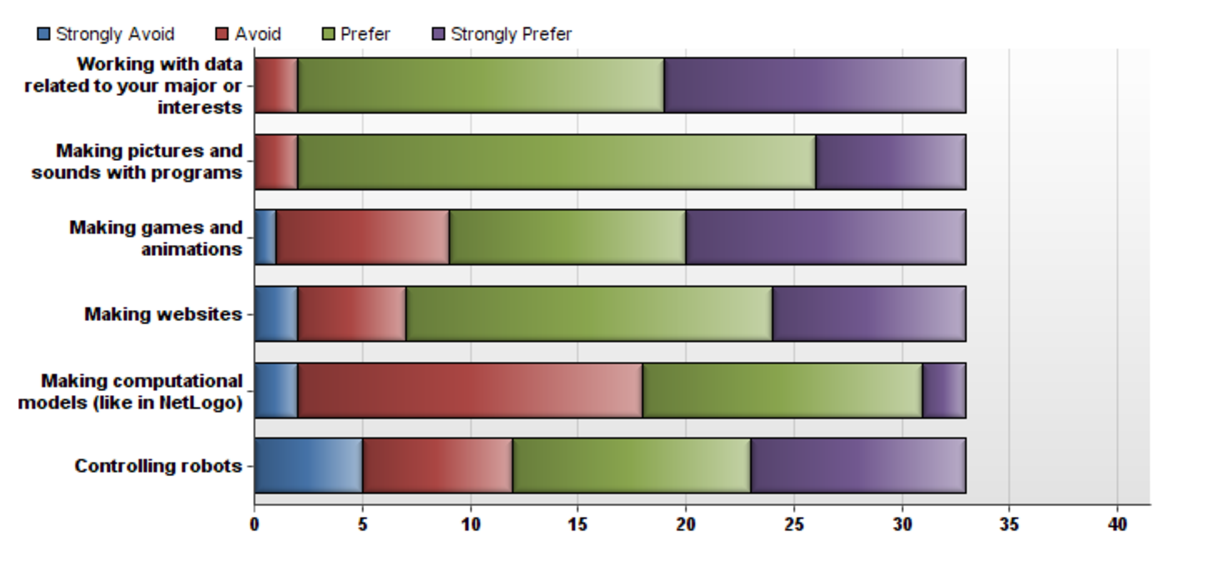
\psfig{file=images/contexts-compared.eps, width=\linewidth}
		\end{center}
		\caption{CT Students' Perceptions of the Appeal of Various Introductory Programming Contexts}
		\label{fig-contexts-compared}
\end{figure}

\begin{figure}
		\begin{center}
				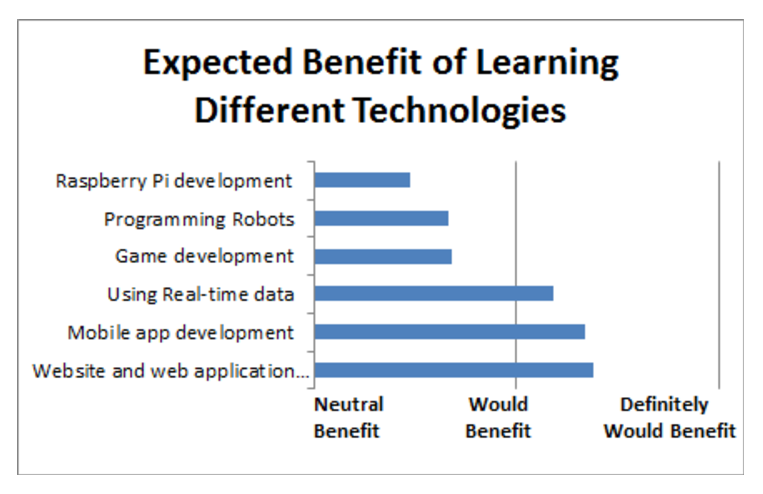
\psfig{file=images/expected-benefit.eps, width=.5\linewidth}
		\end{center}
		\caption{CS Majors' Perceptions of the Benefit of Working with Learning Different Technologies}
		\label{fig-expected-benefit}
\end{figure}

The CORGIS project has been deployed for several semesters in introductory Computer Science courses for majors, ranging from the first course all the way to a Data Structures level course.
These integrations ranged from small assignments to entire semester projects using the software.
So far, the focus of the evaluation has been on the motivational influence of the system.
Quantitative data was collected by surveying students attitudes using well-established motivational frameworks and instruments, and indicates that students tended to find real-time data engaging~\cite{realtimeweb}.
In some courses, qualitative data was gathered through small group interviews, where students attribute increased engagement with the authentic, real-world connection offered by real-time data.

Similar results have been found from its integration in a Computational Thinking course -- students cite working with the realistic data as a key factor in engaging with course materials.
Refer to figure \ref{fig-contexts-compared}, the result of an end-of-course survey (34 responses, 87\% response rate).
Students were asked to respond via a Likert scale to the statement, ``Other schools teach Computational Thinking in different ways. Consider these different styles, and indicate how much you would prefer or avoid them.''
Although this is an extremely shallow question, since students were only exposed to two contexts (computational modelling and working with data), it is an encouraging, preliminary result.

\subsection{Block-Based Programming}

\begin{wrapfigure}{R}{0.5\textwidth}
\label{fig-mlt-overview}
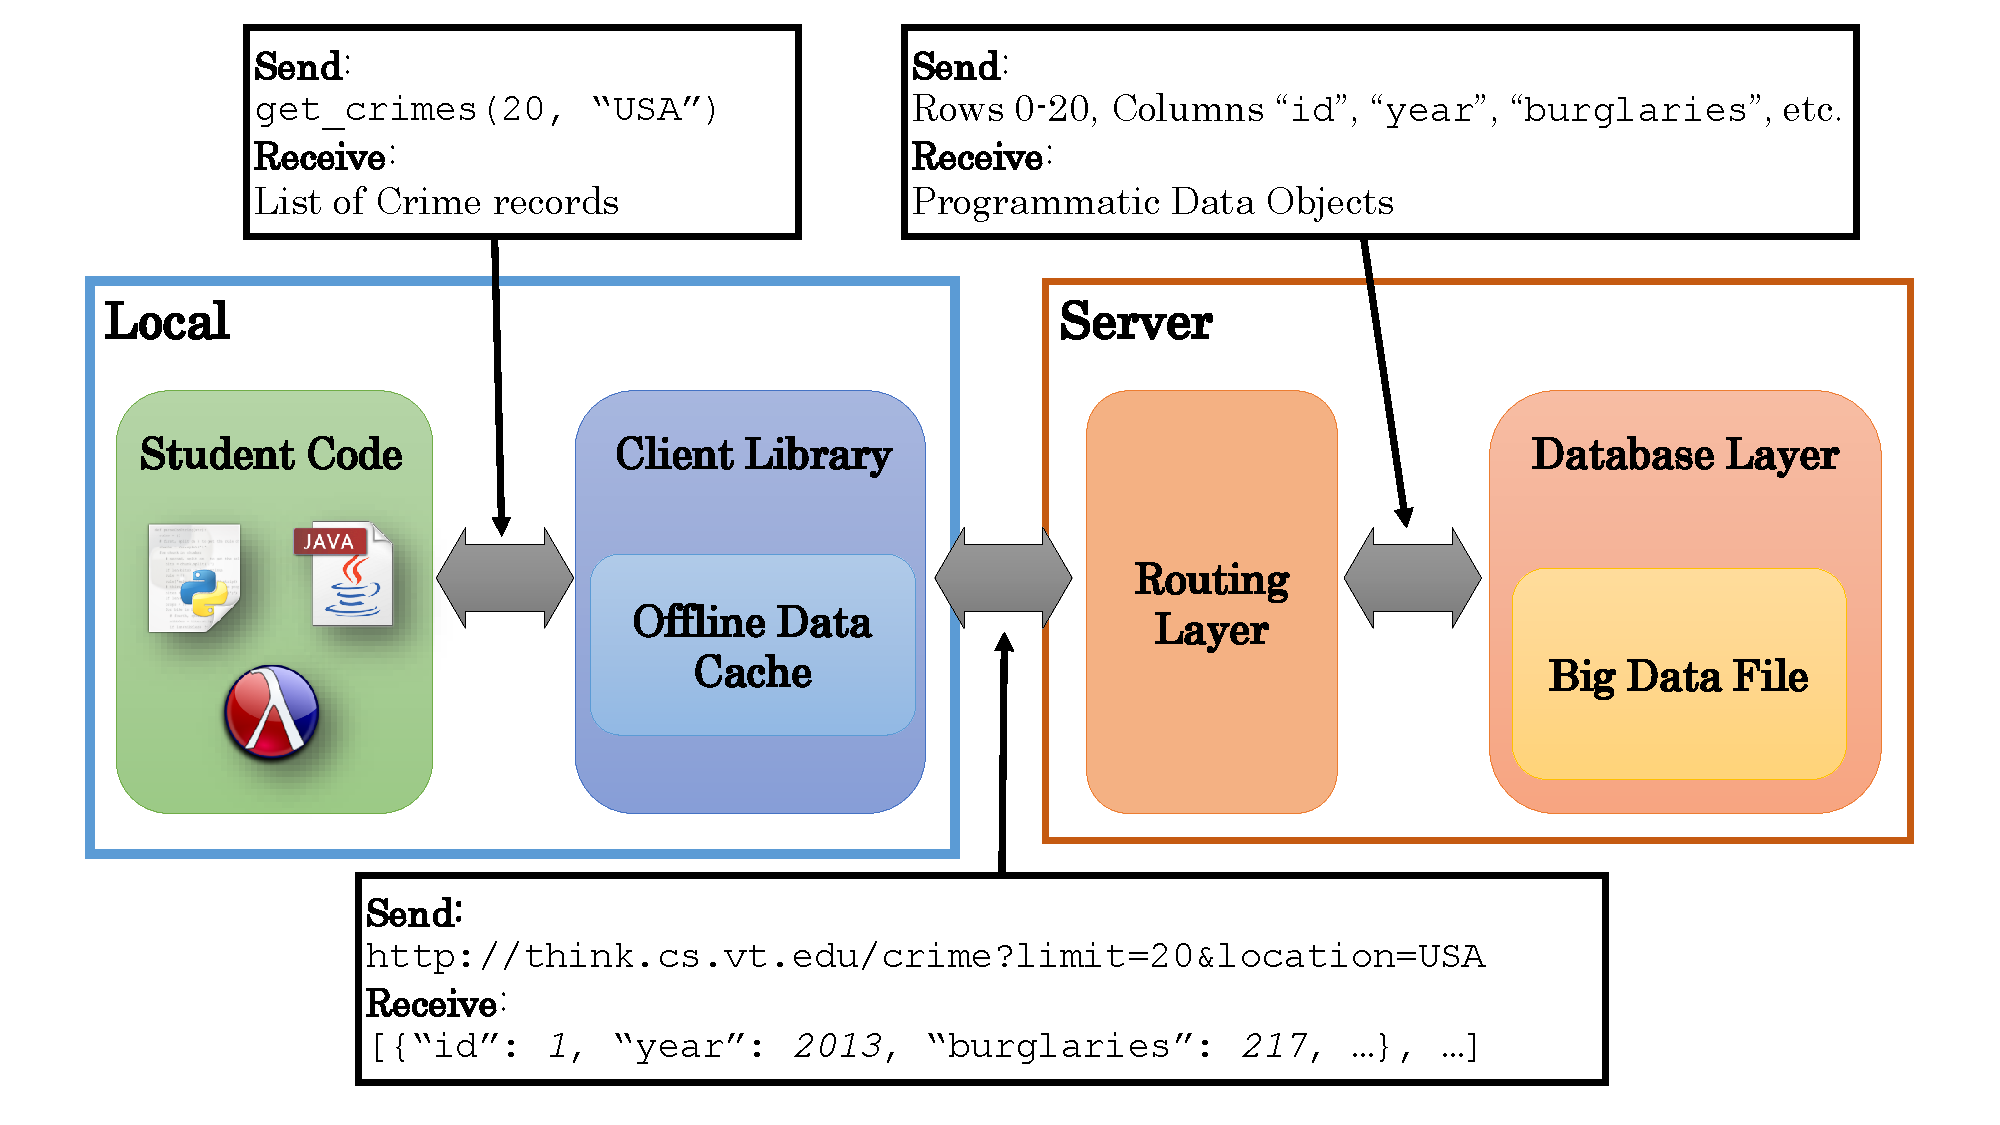
\psfig{file=images/graphics.ps, width=\linewidth}
\caption{The flow of code in the Mutual Language Translation system}
\end{wrapfigure}

Programming is a difficult thing to learn, and there exist many tools to scaffold that process.
One of the more popular approaches is Block-based Programming Environments, which allow the user to build their program from pieces of provided code constructs.
This prevents common syntax errors and some of the the ``blank canvas'' effect.
The CORGIS project has been leveraged in several different block-based environments, including a Python-based system based on Blockly and the popular programming environment/language Snap!. 
Both systems implement their own layer around CORGIS in order to provide access to rich datasets.
The Python/Blockly system has additional tools for creating plotted visualizations of data, and the Snap! interface has generalized support for accessing online data.
Although the Snap! tools were created as part of a spin-off project, the Python/Blockly tools are my own work.

During the Computational Thinking course, students take advantage of the internal caching mechanism of the CORGIS libraries to work on recorded data.
This simplifies the debugging process since programs perform predictably and are no longer dependent on external data services.
When students are ready to run their programs against live data, they can move offline to a traditional programming environment and run in regular production.
This caching mechanism also benefits from an assessment view - a students program can be checked for robustness by invisibly changing the values returned by the big data functions.
Figures \ref{fig-example-blockly} and \ref{fig-example-python} demonstrate the CORGIS library in action both in regular Python code and the equivalent Blockly code.

\begin{figure}
\label{fig-example-blockly}
\label{fig-example-python}
\caption{Blockly vs. Python Code}
\centering
\begin{minipage}[b]{.75\linewidth}
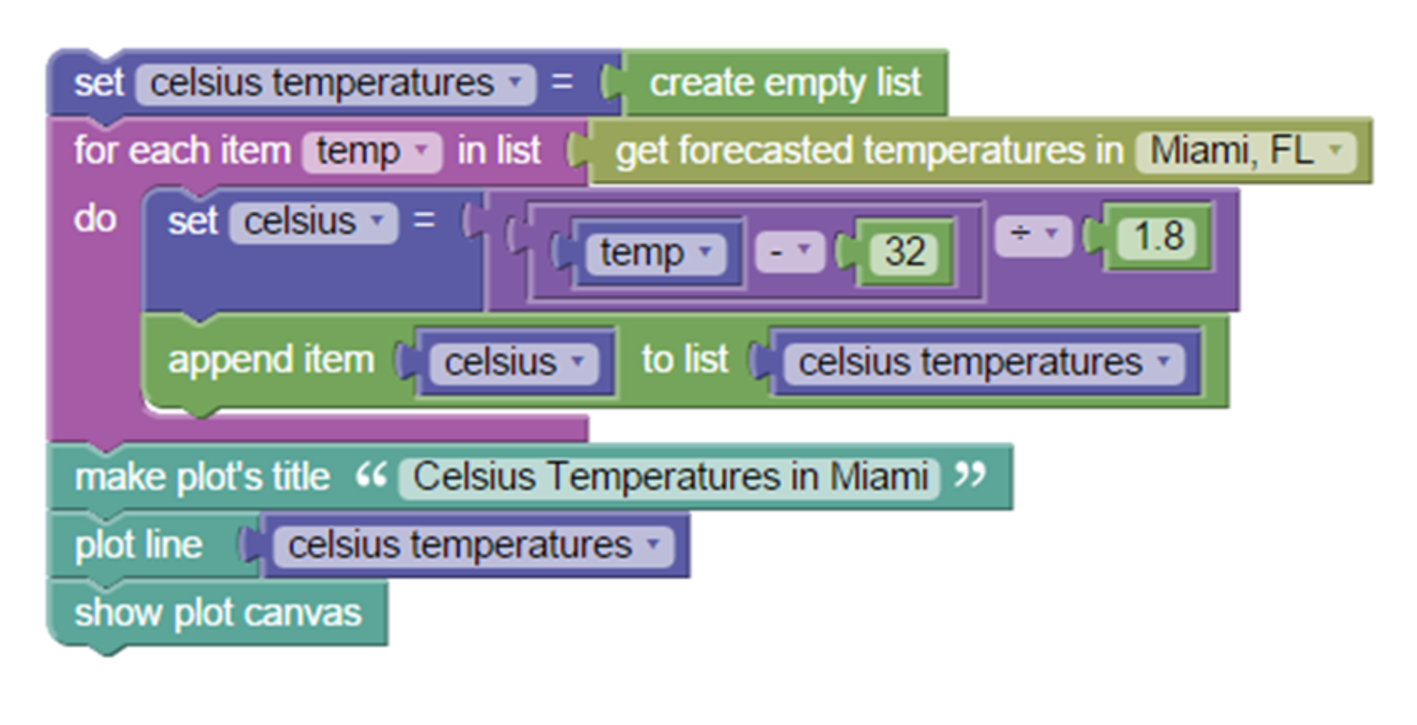
\psfig{file=images/blockly-example.eps, width=\linewidth}
\end{minipage}

\smallskip

\begin{minipage}[b]{.75\linewidth}
\begin{python}
import weather
import matplotlib.pyplot as plt

celsius_temperatures = []
for t in weather.get_temperatures("Miami, FL"):
	celsius = (t - 32) / 1.8
	celsius_temperatures.append(celsius)
plt.title("Celsius Temperatures in Miami")
plt.plot(celsius_temperatures)
plt.show()
\end{python}
\end{minipage}
\end{figure}


\subsubsection{Authenticity of Data}

Careful consideration must be made when choosing problems and designing contexts so that the data leads to optimally authentic learning experiences.
In practice, datasets can vary greatly in authenticity -- some data is collected incorrectly or has other errors, some data was predicted from a model rather than observed from real phenomenon.
A curious component of authenticity, however, is that it is a function of the observer.
A persuasive instructor might convince a class of students that an entirely artificial dataset was representative of real-world data, especially if it confirmed students' existing biases.
There are ethical issues with artificial datasets and the stories that they tell.
However, there are serious pedagogical benefits to generating datasets that fit instructor's goals -- data that leads to interesting visualizations, or clean results.
An important facet of my research will be exploring the ethical and pedagogical ramifications of the authenticity of datasets.

One of the big dangers when attempting to create meaningful context for learners is the problem of \textit{Preauthentication}: attempting to design for authenticity without sufficient knowledge of the audience. This is a problem shared by any approach to introductory material. Petraglia gives a compelling example \cite{preauthentication}:
	
\begin{quotation}
    The task of balancing a checkbook, for instance, may be an authentic task from the perspective of a 21-year-old, but we would question its authenticity from the perspective of a 5-year-old. But more to the point, even among 21-year-olds, for whom we believe the task should be authentic, there are some who will find any given lesson in personal finance irrelevant, inaccurate, or otherwise inappropriate. 
\end{quotation}
Preauthentication stems from over-generalizations and run-away assumptions.
If you attempt to reduce an entire classroom to a list of likes and dislikes, you run the risk of ignoring each individual learner's rich history and background that they will be building from. 
It is difficult to plan for and work against this ever-present danger when designing reusable assignments. 
Petraglia \cite{preauthentication} recommends that rather than attempting to design around students prior understanding, it is better to simply convince the learner of the authenticity of the problem.
But this is limiting, since it ignores the prior experiences and understanding that a student brings to their learning.
Instead, it would be better to find a middle ground where students are given flexibility while maintaining a relatively uniform experience for students.
In an ideal learning environment, students will have freedom to explore datasets of their own choosing, possibly from a list.
Of course, this must be balanced with the students inexperience with finding datasets, requiring the process be given time and attention.
